\begin{sol}
    Similar to the dihedral group of a square, adjacent vertices must remain adjacent after a symmetric transformation. Unlike the case of a square, we propose that the symmetry $\sigma$ is now uniquely defined by:
    \begin{equation}
        (\sigma(1), \sigma(2), \sigma(3)) = (x,y,z)
    \end{equation}
    where $2$ and $3$ are adjacent to $1$, as shown below:
    \begin{center}
    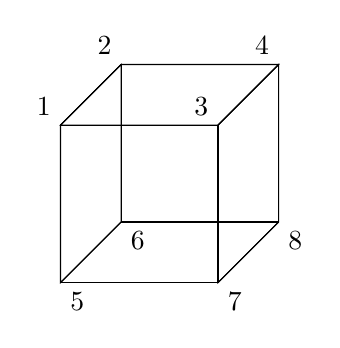
\begin{tikzpicture}[
      ]
      \def\Side{2}
      \coordinate (A1) at (0,0,0);
      \coordinate (A2) at (0,\Side,0);
      \coordinate (A3) at (\Side,\Side,0);
      \coordinate (A4) at (\Side,0,0);
      \coordinate (B1) at (0,0,\Side);
      \coordinate (B2) at (0,\Side,\Side);
      \coordinate (B3) at (\Side,\Side,\Side);
      \coordinate (B4) at (\Side,0,\Side);
      
      \draw (A2) -- (A3) -- (B3) -- (B2) -- cycle;
      \draw  (A2) -- (A3) -- (A4) -- (A1) -- cycle;
      \draw(A3) -- (B3) -- (B4) -- (A4) -- cycle;
      \draw   (A1) -- (A2) -- (B2) -- (B1) -- cycle;
      
      \draw (A2) -- (A1) -- (A4);
      \draw (B2) -- (B1) -- (B4) -- (B3) -- cycle;
      \draw (A1) -- (B1);
      \draw (A2) -- (B2);
      \draw (A4) -- (B4);
      
      \draw[thin] (A3) -- (B3);
      \draw[thin] (A3) -- (A4);
    
      
      \node[above left] at (B2) {$1$};
      \node[above left] at (A2) {$2$};
      \node[above left] at (B3) {$3$};
      \node[above left] at (A3) {$4$};
      
      \node[below right] at (B1) {$5$};
      \node[below right] at (A1) {$6$};
      \node[below right] at (B4) {$7$};
      \node[below right] at (A4) {$8$};
      \end{tikzpicture}
    \end{center}
    \begin{proof}
        Every vertex is adjacent to three vertices. We know that $y$ and $z$ are adjacent to $x$, so we can determine the third vertex adjacent to $x$, which we will call $a=\sigma(5)$. Each of the three pairs of vertices in the set $\{y,z,a\}$ are on a face diagonal, where the face contains the vertex $x$.
        \vspace{2mm}

        For each vertex $v_i$, there exists only one other vertex $v_j$ that is the furthest apart from it, and it always occurs at the opposite end. We will denote such a $(v_i,v_j)$ as an \textit{enemy pair}. Since symmetries preserve distances and we know the locations of vertices $a,y,z$ who are all adjacent to $x$ (no pair of the known vertices form an enemy pair) we can uniquely determine each vertex's enemy pair and therefore the locations of all eight vertices.
    \end{proof}
    We have eight choices for $x$, three choices for $y$, and two choices for $z$ for a total of $8\times 3\times 2 = 48$ symmetries.
\end{sol}